\documentclass{report}
\usepackage[format = hang, font = bf]{caption}
\usepackage{subcaption}
% The following is needed in order to make the code compatible
% with both latex/dvips and pdflatex. Added for using UML generated by MetaUML.
\ifx\pdftexversion\undefined
\usepackage[dvips]{graphicx}
\else
\usepackage[pdftex]{graphicx}
\DeclareGraphicsRule{*}{mps}{*}{}
\fi
\usepackage{array}
\usepackage{amsmath}
\usepackage{amsthm}
\usepackage{mathtools}
\usepackage{boxedminipage}
\usepackage{listings}
\usepackage{multicol}
\usepackage{makecell}%diagonal line in table
\usepackage{float}%allowing forceful figure[H]
\usepackage{xcolor}
\usepackage{mathrsfs}%mathcal
\usepackage{amsfonts}%allowing \mathbb{R}
\usepackage{amssymb}
\usepackage{alltt}
\usepackage{algorithmicx}
\usepackage[chapter]{algorithm} 
%chapter option ensures that algorithms are numbered within each chapter rather than in the whole article
\usepackage[noend]{algpseudocode} %If end if, end procdeure, etc is expected to appear, remove the noend option
\usepackage{xspace}
\usepackage{physics}
\usepackage{color}
\usepackage{tikz}
\usetikzlibrary{shapes,positioning}
\usepackage{url}
\def\UrlBreaks{\do\A\do\B\do\C\do\D\do\E\do\F\do\G\do\H\do\I\do\J\do\K\do\L\do\M\do\N\do\O\do\P\do\Q\do\R\do\S\do\T\do\U\do\V\do\W\do\X\do\Y\do\Z\do\[\do\\\do\]\do\^\do\_\do\`\do\a\do\b\do\c\do\d\do\e\do\f\do\g\do\h\do\i\do\j\do\k\do\l\do\m\do\n\do\o\do\p\do\q\do\r\do\s\do\t\do\u\do\v\do\w\do\x\do\y\do\z\do\0\do\1\do\2\do\3\do\4\do\5\do\6\do\7\do\8\do\9\do\.\do\@\do\\\do\/\do\!\do\_\do\|\do\;\do\>\do\]\do\)\do\,\do\?\do\'\do+\do\=\do\#\do\-}
\usepackage{xr}%allow cross-file references
\usepackage[breaklinks = true]{hyperref}
\usepackage{thmtools}
\lstset{
language = C++, 
showspaces = false,
breaklines = true, 
tabsize = 2, 
numbers = left, 
extendedchars = false, 
basicstyle = {\ttfamily \footnotesize}, 
keywordstyle=\color{blue!70}, 
commentstyle=\color{gray}, 
frame=shadowbox, 
rulesepcolor=\color{red!20!green!20!blue!20}, 
numberstyle={\color[RGB]{0,192,192}}, 
moredelim=[is][\underbar]{_}{_}
}
\mathchardef\myhyphen="2D
% switch-case environment definitions
\algblock{switch}{endswitch} 
\algblock{case}{endcase}
%\algrenewtext{endswitch}{\textbf{end switch}} %If end switch is expected to appear, uncomment this line.
\algtext*{endswitch} % Make end switch disappear
\algtext*{endcase}
\algnewcommand\algorithmicinput{\textbf{Input}}
\algnewcommand\Input{\item[\algorithmicinput]}
\algnewcommand\algorithmicoutput{\textbf{Output}}
\algnewcommand\Output{\item[\algorithmicoutput]}
\algnewcommand\algorithmicinputoutput{\textbf{input and output:}}
\algnewcommand\InputOutput{\item[\algorithmicinputoutput]}
\allowdisplaybreaks
\newtheorem{theorem}{Theorem}
\newtheorem{corollary}[theorem]{Corollary}
\newtheorem{lemma}[theorem]{Lemma}
\newtheorem{definition}{Definition}
\renewcommand{\listtheoremname}{List of Important Theorems}
\def\PREAMBLE{PREAMBLE}
\title{Notes for Cryptography}
\author{Jing LI\\pkuyplijing@gmail.com}
\begin{document}
\pagestyle{empty}
\hypersetup{pageanchor=false}
\maketitle
\begin{center}
\emph{Sincere gratitude to Professor Dan Boneh\\for offering such a wonderful course.}
\end{center}
\tableofcontents
\newpage
\hypersetup{pageanchor=true}
\pagenumbering{arabic}
\pagestyle{headings}
\addtocontents{toc}{\protect\thispagestyle{empty}}
\ifx\PREAMBLE\undefined
\documentclass{report}
\usepackage[format = hang, font = bf]{caption}
\usepackage{subcaption}
% The following is needed in order to make the code compatible
% with both latex/dvips and pdflatex. Added for using UML generated by MetaUML.
\ifx\pdftexversion\undefined
\usepackage[dvips]{graphicx}
\else
\usepackage[pdftex]{graphicx}
\DeclareGraphicsRule{*}{mps}{*}{}
\fi
\usepackage{array}
\usepackage{amsmath}
\usepackage{amsthm}
\usepackage{mathtools}
\usepackage{boxedminipage}
\usepackage{listings}
\usepackage{multicol}
\usepackage{makecell}%diagonal line in table
\usepackage{float}%allowing forceful figure[H]
\usepackage{xcolor}
\usepackage{mathrsfs}%mathcal
\usepackage{amsfonts}%allowing \mathbb{R}
\usepackage{amssymb}
\usepackage{alltt}
\usepackage{algorithmicx}
\usepackage[chapter]{algorithm} 
%chapter option ensures that algorithms are numbered within each chapter rather than in the whole article
\usepackage[noend]{algpseudocode} %If end if, end procdeure, etc is expected to appear, remove the noend option
\usepackage{xspace}
\usepackage{physics}
\usepackage{color}
\usepackage{tikz}
\usetikzlibrary{shapes,positioning}
\usepackage{url}
\def\UrlBreaks{\do\A\do\B\do\C\do\D\do\E\do\F\do\G\do\H\do\I\do\J\do\K\do\L\do\M\do\N\do\O\do\P\do\Q\do\R\do\S\do\T\do\U\do\V\do\W\do\X\do\Y\do\Z\do\[\do\\\do\]\do\^\do\_\do\`\do\a\do\b\do\c\do\d\do\e\do\f\do\g\do\h\do\i\do\j\do\k\do\l\do\m\do\n\do\o\do\p\do\q\do\r\do\s\do\t\do\u\do\v\do\w\do\x\do\y\do\z\do\0\do\1\do\2\do\3\do\4\do\5\do\6\do\7\do\8\do\9\do\.\do\@\do\\\do\/\do\!\do\_\do\|\do\;\do\>\do\]\do\)\do\,\do\?\do\'\do+\do\=\do\#\do\-}
\usepackage{xr}%allow cross-file references
\usepackage[breaklinks = true]{hyperref}
\usepackage{thmtools}
\lstset{
language = C++, 
showspaces = false,
breaklines = true, 
tabsize = 2, 
numbers = left, 
extendedchars = false, 
basicstyle = {\ttfamily \footnotesize}, 
keywordstyle=\color{blue!70}, 
commentstyle=\color{gray}, 
frame=shadowbox, 
rulesepcolor=\color{red!20!green!20!blue!20}, 
numberstyle={\color[RGB]{0,192,192}}, 
moredelim=[is][\underbar]{_}{_}
}
\mathchardef\myhyphen="2D
% switch-case environment definitions
\algblock{switch}{endswitch} 
\algblock{case}{endcase}
%\algrenewtext{endswitch}{\textbf{end switch}} %If end switch is expected to appear, uncomment this line.
\algtext*{endswitch} % Make end switch disappear
\algtext*{endcase}
\algnewcommand\algorithmicinput{\textbf{Input}}
\algnewcommand\Input{\item[\algorithmicinput]}
\algnewcommand\algorithmicoutput{\textbf{Output}}
\algnewcommand\Output{\item[\algorithmicoutput]}
\algnewcommand\algorithmicinputoutput{\textbf{input and output:}}
\algnewcommand\InputOutput{\item[\algorithmicinputoutput]}
\allowdisplaybreaks
\newtheorem{theorem}{Theorem}
\newtheorem{corollary}[theorem]{Corollary}
\newtheorem{lemma}[theorem]{Lemma}
\newtheorem{definition}{Definition}
\renewcommand{\listtheoremname}{List of Important Theorems}
\begin{document}
\fi
\chapter{Introduction}
\section{Course Overview}
The main objectives of this course are 
\begin{itemize}
\item Learn how cryptographic primitives work;
\item Learn how to use them correctly and reason about security.
\end{itemize}
By the end of the course we will be able to reason about the security of cryptography constructions and break ones that are not secure. 

Cryptography is used everywhere.
\begin{description}
\item[Secure communication] Web traffic: https. Wireless traffic: 802.11i WPA2, GSM, Bluetooth.
\item[Encrypting files on disk] EFS, TrueCrypt
\item[Content protection(e.g. DVD, blue ray)] CSS(Content Scrambling System), AACS
\item[User authentication]
\end{description}

Secure communication is concerned about a laptop ``Alice'' trying to communicate with a web server ``Bob''
\footnote{Alice and Bob are two nicknames that will be used in the course}. The protocol used is HTTPS, or to say SSL(Secure Sockets Layer)/TLS(Transport Layer Security). The goal is to make sure that as data travels across the network, an attacker can neither eavesdrop on or tamper the data. It consists of two parts: 
\begin{itemize}
\item Handshake protocol: establish a shared secret key using public-key cryptography;
\item Record layer: transmit data using this shared secret key, with confidentiality and integrity ensured.
\end{itemize}

Storing encrypted files on disk is actually logically the same as protecting communication: encrypting files on disk is essentially securing the communication between ``Alice today'' and ``Alice tomorrow''. 

The building block of secure communication is symmetric encryption. A message $m$ is encrypted by a cipher using a shared key $k$ into a cipher text $c=E(k,m)$, and this cipher text is deciphered back to the message: $m=D(k,c)$. The encryption algorithm $E$ and the decryption algorithm $D$ are publicly known. Proprietary ciphers should not be used for security reasons.

We will discuss two use cases of symmetric encryption. A single use key is used to encrypt only one message, while a multi use key is used to encrypt multiple messages. 

Cryptography is a tremendous tool serving as the basis for many security mechanisms. Nonetheless, it is not the solution to all security problems. Software bugs can cause security problems unsolvable using cryptography. Neither can cryptography prevent us from social engineering attacks. Moreover, cryptography is not reliable unless implemented and used properly. It is not something we try to invent ourselves. 

\section{What is Cryptography}
As stated in the previous section, the core of cryptography consists of two steps: secret key establishment and secure communication using the secret key. But cryptography does much more than that. We will provide a few examples here. 
\subsubsection{Digital Signature}
Digital signature is the analog of the signature in the physical world. In the digital world, signatures cannot be the same for different documents. Rather, digital signature is a function of the content beings signed. Simply copying the signature on one document onto another one will result in failure of verification.
\subsubsection{Anonymous Communication}
Anonymous communication over the Internet can be established with a commonly used mechanism called ``mix net''. Bob has no idea to whom he is talking when Alice contacts him anonymously, yet he can still respond to Alice.
\subsubsection{Anonymous Digital Cash}
The use of digital cash is concerned with two problems: how to spend a ``digital coin'' without anyone knowing who I am, and how to prevent double spending. There seems to be a paradox between anonymity and security. Roughly speaking, anonymous digital cash is used in such a way that when used once, no one knows who used it, whilst once used twice, the identity of the user gets exposed. 
\subsubsection{Protocols}
In a election, we may hope to design a system that reveals the winner of the election without exposing individual voting choices. In a private auction, it is ideal that only the winner and the 2$^{nd}$ highest bid is outputted by the auction center. These are actually examples of a more general problem called secure multi-party computation. It aims at calculating a target function $f(x_i)$ without exposing individual inputs $x_i$.
\subsubsection{``Crypto Magic''}
\begin{itemize}
\item Privately outsourcing computation: send an encrypted query to Google, and Google can compute on the encrypted query and send back results without knowing content of the query.
\item Zero knowledge proof: convince someone else that we have solved a problem without exposing the solution to him. 
\end{itemize}
Cryptography is a rigorous science. Every concept that we will describe is going to follow three steps: 
\begin{enumerate}
\item Precisely specify the threat model;
\item Propose a construction;
\item Prove that breaking the construction under the threat model is equivalent to solving an underlying hard problem.
\end{enumerate}

\section{History of Cryptography}
We will provide a few historical ciphers, all of which are now badly broken. 
\subsubsection{Substitution Cipher}
Cipher a piece of text by substituting each letter with another letter, i.e. encrypt messages by shuffling the alphabet. An example of substitution cipher is the Caesar cipher. It shifts the alphabet by 3 positions, i.e. $a\rightarrow d, b\rightarrow e$, etc. 

There are 26! possible keys for a substitution cipher, which is a fairly large key space. However it can be easily broken with letter frequencies. Being vulnerable to the worst possible attack, namely a cipher text only attack, it should not be the choice of any serious secure communication.
\subsubsection{Vigener Cipher}
A cipher dating back to 16$^{th}$-century Rome. Given a key word, for example ``crypto''. Repeat the word enough times until reaching the length of the message, then add the long key with the message numerically to obtain the cipher text. It can also be broken with letter frequencies. 
\subsubsection{Rotor Machines}
A cipher invented during the electric era, i.e. the 19$^{th}$ century. The most famous one was the Enigma.
\subsubsection{Data Encryption Standard}
A post-WWII cipher with a key space of size $2^{56}$, which was large enough then but is too small today. 
\section{Discrete Probability}
The whole theory of cryptography is built upon the knowledge of discrete probability. This section serves as a quick recap of discrete probability.

Discrete probability is always defined on a finite set called the \textbf{universe}. In this course we will always use the set $U=\{0,1\}^n$, i.e. the set of all $n$-bit binary strings.
\begin{definition}
A \textbf{probability distribution} $P$ is a function from $U$ to [0,1] such that $\sum\limits_{x\in U}P(x)=1$.
\end{definition}
\begin{definition}
A subset of the universe $A\subseteq U$ is called an \textbf{event}. The probability of the event is $Pr(A)=\sum\limits_{x\in A}P(x)\in[0,1]$.
\end{definition}
\begin{theorem}(\textbf{The Union Bound})
\[Pr(A_1 \cup A_2)\le Pr(A_1)+Pr(A_2)\]
\end{theorem}
\begin{definition}
A \textbf{random variable} is a function $X:U\rightarrow V$. $X$ takes values in $V$ and defines a distribution on $V$.
\end{definition}
\begin{definition}A \textbf{uniform random variable} over $U$, denoted as $r\xleftarrow{\text{R}} U$, has the property that 
\[Pr(r = a)=\frac{1}{\lvert U\rvert}\]
for all $a\in U$.
\end{definition}

A deterministic algorithm obtains the same result every time as long as the input is the same:$y\leftarrow A(m)$, whereas a randomized algorithm that takes an implicit argument sampled anew each time obtains a different result each time with the same input: $y\leftarrow A(m;r),\text{ where } r\xleftarrow{R}\{0,1\}^n$. Actually the output of a randomized algorithm can be thought of as a random variable: $y\xleftarrow{R}A(m)$.

\begin{definition}
Events $A$ and $B$ are \textbf{independent} if \
\[Pr(A\land B)=Pr(A)\cdot Pr(B)\]
\end{definition}

An important property of XOR will be frequently used in this course.
\begin{theorem}\textbf{(Property of XOR)}
Suppose we have a random variable $Y$ and a uniform variable $X$ independent from $Y$ on $\{0,1\}^n$, then the XOR of $X$ and $Y$ $Z\coloneqq X\oplus Y$ is a uniform variable on $\{0,1\}^n$.
\end{theorem}
\begin{proof}(for $n$=1)
\begin{equation*}
\begin{split}
Pr(Z=0) &=Pr(X=0)\cdot Pr(Y=0) + Pr(X=1)\cdot Pr(Y=1)\\
        &=\frac{1}{2}\left(Pr(X=0) + Pr(X=1)\right)=\frac{1}{2}
\end{split}
\end{equation*}
\end{proof}

The birthday paradox is an interesting topic that we will talk about in detail later.
\begin{theorem}\textbf{(The Birthday Paradox)}
Let $r_i\in U(i=1,\dots,n)$ be independent identically distributed variables. If $n\geq 1.2\times\lvert U\rvert^{1/2}$, then 
\[Pr(\exists i\neq j\:s.t.\:r_i=r_j)\geq\frac{1}{2}\]
\end{theorem}
\ifx\PREAMBLE\undefined
\end{document}
\fi
\ifx\PREAMBLE\undefined
\documentclass{report}
\usepackage[format = hang, font = bf]{caption}
\usepackage{subcaption}
% The following is needed in order to make the code compatible
% with both latex/dvips and pdflatex. Added for using UML generated by MetaUML.
\ifx\pdftexversion\undefined
\usepackage[dvips]{graphicx}
\else
\usepackage[pdftex]{graphicx}
\DeclareGraphicsRule{*}{mps}{*}{}
\fi
\usepackage{array}
\usepackage{amsmath}
\usepackage{amsthm}
\usepackage{mathtools}
\usepackage{boxedminipage}
\usepackage{listings}
\usepackage{multicol}
\usepackage{makecell}%diagonal line in table
\usepackage{float}%allowing forceful figure[H]
\usepackage{xcolor}
\usepackage{mathrsfs}%mathcal
\usepackage{amsfonts}%allowing \mathbb{R}
\usepackage{amssymb}
\usepackage{alltt}
\usepackage{algorithmicx}
\usepackage[chapter]{algorithm} 
%chapter option ensures that algorithms are numbered within each chapter rather than in the whole article
\usepackage[noend]{algpseudocode} %If end if, end procdeure, etc is expected to appear, remove the noend option
\usepackage{xspace}
\usepackage{physics}
\usepackage{color}
\usepackage{tikz}
\usetikzlibrary{shapes,positioning}
\usepackage{url}
\def\UrlBreaks{\do\A\do\B\do\C\do\D\do\E\do\F\do\G\do\H\do\I\do\J\do\K\do\L\do\M\do\N\do\O\do\P\do\Q\do\R\do\S\do\T\do\U\do\V\do\W\do\X\do\Y\do\Z\do\[\do\\\do\]\do\^\do\_\do\`\do\a\do\b\do\c\do\d\do\e\do\f\do\g\do\h\do\i\do\j\do\k\do\l\do\m\do\n\do\o\do\p\do\q\do\r\do\s\do\t\do\u\do\v\do\w\do\x\do\y\do\z\do\0\do\1\do\2\do\3\do\4\do\5\do\6\do\7\do\8\do\9\do\.\do\@\do\\\do\/\do\!\do\_\do\|\do\;\do\>\do\]\do\)\do\,\do\?\do\'\do+\do\=\do\#\do\-}
\usepackage{xr}%allow cross-file references
\usepackage[breaklinks = true]{hyperref}
\usepackage{thmtools}
\lstset{
language = C++, 
showspaces = false,
breaklines = true, 
tabsize = 2, 
numbers = left, 
extendedchars = false, 
basicstyle = {\ttfamily \footnotesize}, 
keywordstyle=\color{blue!70}, 
commentstyle=\color{gray}, 
frame=shadowbox, 
rulesepcolor=\color{red!20!green!20!blue!20}, 
numberstyle={\color[RGB]{0,192,192}}, 
moredelim=[is][\underbar]{_}{_}
}
\mathchardef\myhyphen="2D
% switch-case environment definitions
\algblock{switch}{endswitch} 
\algblock{case}{endcase}
%\algrenewtext{endswitch}{\textbf{end switch}} %If end switch is expected to appear, uncomment this line.
\algtext*{endswitch} % Make end switch disappear
\algtext*{endcase}
\algnewcommand\algorithmicinput{\textbf{Input}}
\algnewcommand\Input{\item[\algorithmicinput]}
\algnewcommand\algorithmicoutput{\textbf{Output}}
\algnewcommand\Output{\item[\algorithmicoutput]}
\algnewcommand\algorithmicinputoutput{\textbf{input and output:}}
\algnewcommand\InputOutput{\item[\algorithmicinputoutput]}
\allowdisplaybreaks
\newtheorem{theorem}{Theorem}
\newtheorem{corollary}[theorem]{Corollary}
\newtheorem{lemma}[theorem]{Lemma}
\newtheorem{definition}{Definition}
\renewcommand{\listtheoremname}{List of Important Theorems}
\begin{document}
\fi
\chapter{Stream Ciphers}
First we would like to provide a precise definition for symmetric ciphers.
\begin{definition}\textbf{(Symmetric Cipher)}
A \textbf{cipher} defined over $(\mathcal{K,M,C})$, in which $\mathcal{K}$ is the set of all possible keys, $\mathcal{M}$ is the set of all possible messages and $\mathcal{C}$ is the set of all possible cipher texts, is a pair of efficient algorithms $(E,D)$ in which the encryption algorithm $E:\mathcal{K\times M}\rightarrow\mathcal{C}$ and the decryption algorithm $D:\mathcal{K\times C}\rightarrow \mathcal{M}$ satisfy the consistence equation
\begin{equation*}
D(k,E(k,m))=m, \forall k\in\mathcal{K},m\in\mathcal{M}.
\end{equation*}
\end{definition}
In practice, $E$ is often randomized, while $D$ is always deterministic.
\section{One Time Pad and Perfect Secrecy}
Now we will introduce our first example of a secure cipher, namely \textbf{the one time pad}. In this case, we have $\mathcal{K=M=C=}\{0,1\}^n$. A key is simply a bit string with the same length as the message text. The cipher text is the XOR of the key and the message, i.e.
\begin{equation*}
c\coloneqq E(k,m)= k\oplus m.
\end{equation*}
To decrypt a cipher text, we simply compute the XOR again, i.e.
\begin{equation*}
m\coloneqq E(k,c)= k\oplus c.
\end{equation*}
Since we have $D(k,E(k,m))=k\oplus(k\oplus m)=(k\oplus k)\oplus m=0\oplus m=m$\footnote{XOR is addition mod 2, thus is associative. Also provable using $a\oplus b=a\cdot\bar{b}+\bar{a}\cdot b$.}, obviously the consistence equation is satisfied. Similarly we have $k=m\oplus c$.

Now let's explain why OTP is a ``good'' cipher.
\begin{definition}\textbf{(Perfect Secrecy)}
A cipher $(E,D)$ over $(\mathcal{K}, \mathcal{M}, \mathcal{C})$ has \textbf{perfect secrecy} if $\forall m_0,m_1\in\mathcal{M}$ with equal length and $\forall c\in\mathcal{C}$, we have 
\begin{equation*}
Pr(E(k,m_0)=c)=Pr(E(k,m_1)=c),
\end{equation*}
in which $k$ is uniform in $\mathcal{K}: k\xleftarrow{R}\mathcal{K}.$
\end{definition}
This definition means that an attacker cannot tell if the message is $m_0, m_1$ or any other message with equal length given only the cipher text. Thus nothing can be learnt about the message from the cipher text, and the cipher is safe from CT-only attack. 

Since $k=c\oplus m$ for OTP, we have $Pr(E(k,m)=c)=\frac{1}{\lvert\mathcal{K}\rvert},\forall c,m$. Hence OTP has perfect secrecy. Nonetheless, the key has to be as long as the message, which makes OTP impractical in actual use. 

Unfortunately, it can be proved that a cipher with perfect secrecy must satisfy $\lvert\mathcal{K}\rvert\ge\lvert\mathcal{M}\rvert$, which means that the length of the key is at least as long as that of the message. So such ciphers are actually hard to use in practice.
\section{Stream Ciphers}
In this section we will try to make OTP practical. The idea is to use a pseudo-random key instead of a random key. 
\begin{definition} \textbf{(PRG)}
A \textbf{pseudo-random generator} is a function $G:\{0,1\}^s\rightarrow\{0,1\}^n$, in which $n\gg s$. 
\end{definition}
$\{0,1\}^s$ is called the \textbf{seed space}. A PRG must be efficiently computable by a deterministic algorithm. A \textbf{stream cipher} just substitutes the random key in OTP with a pseudo-random key generated by a PRG, i.e. with a random seed $k\in\{0,1\}^s$, we have
\begin{align*}
c=E(k,m)=m\oplus G(k)\\
m=D(k,m)=c\oplus G(k)
\end{align*}

Obviously a stream cipher cannot have perfect secrecy because the seed is much shorter than the message. Thus we need a different notion of security, and the security of a stream cipher depends on the PRG used. 

If an attacker is able to compute all bits of $G(k)$ according to the first $i$ bits, then the PRG is not safe from CT-only attacks. For example, an email following the SMTP protocol always starts with ``from:'', thus the attacker can obtain a prefix of $G(k)$ according to the cipher text. We should always use \textbf{unpredictable PRGs} as defined below.
\begin{definition}\textbf{(Predictable PRG)}
A PRG $G$ is \textbf{predictable} if $\exists$ efficient algorithm $\mathcal{A}$ and $i\in[1,n-1]$ s.t. 
\begin{equation*}
Pr\left(\mathcal{A}\left(\left.G(k)\right\vert_{1,\dots,i}\right)=\left.G(k)\right\vert_{i+1}\right)\geq\frac{1}{2}+\epsilon
\end{equation*}
in which $G(k)\vert_{i,...,j}$ is the $i^{th}$ to the $j^{th}$ bit of ${G(k)}$, for some non-negligible $\epsilon$. 
\end{definition}
\begin{definition}\textbf{(Unpredictable PRG)}
A PRG is \textbf{unpredictable} if it is not predictable. 
\end{definition}
An example of predictable PRG is the famous \textbf{linear congruential generator}. A seed $r[0]$ is chosen randomly. Then we calculate
\begin{equation*}
r[i]=(a\cdot r[i-1]+b)\bmod p
\end{equation*}
in which $a,b$ are integer parameters and $p$ is a prime number. In each iteration a few bits of $r[i]$ is outputted. This PRG is easy to predict. 

A variant is the \texttt{random()} function in glibc:
\begin{equation*}
r[i]=(r[i-3]+r[i-31])\%2^{32}
\end{equation*}
and output $r[i]\gg 1$. \texttt{random()} should never be used for cryptography.

A theoretical notion of negligibility is to view $\epsilon$ as a function rather than a scalar. $\epsilon:Z^+\rightarrow R^+$ is non-negligible if $\exists d$ s.t. $\epsilon(\lambda)\geq\frac{1}{\lambda^d}$ is infinitely often, i.e. $\epsilon$ is larger than $\frac{1}{\text{polynomial of }\lambda}$ for many $\lambda$. On the contrary, $\epsilon$ is negligible if $\forall d,\exists \lambda_d$ s.t. $\epsilon(\lambda)\leq\frac{1}{\lambda^d},\forall\lambda\geq\lambda_d.$ For instance, $\frac{1}{2^\lambda}$ is negligible, whilst $\frac{1}{\lambda^{1000}}$ is non-negligible. As a tricky example, 
\[\epsilon(\lambda)=\begin{cases}
\frac{1}{2^\lambda}&\text{for odd }\lambda\\
\frac{1}{\lambda^{1000}}&\text{for even }\lambda
\end{cases}\]
is non-negligible.
\section{Attacks on OTP and Stream Ciphers}
\subsection{Two Time Pad}
A pad should not be used more than once, otherwise the encrypted messages shall be decrypted easily. Suppose two messages $m_1,m_2$ are encrypted using the same pad $PRG(k)$:
\begin{align*}
c_1\leftarrow m_1\oplus PRG(k)\\
c_2\leftarrow m_2\oplus PRG(k)
\end{align*}
If an eavesdropper has intercepted the two cipher texts. By calculating their XOR:
\begin{align*}
c_1\oplus c_2&=(m_1\oplus PRG(k))\oplus(m_2\oplus PRG(k))\\
&=m_1\oplus(PRG(k)\oplus PRG(k))\oplus m_2\\
&=m_1\oplus 0\oplus m_2=m_1\oplus m_2
\end{align*}
The English language and the ASCII encoding has enough redundancy so that $m_1$ and $m_2$ can be easily decoded from $m_1\oplus m_2$. Examples of the use of two time pads are not rare in the real world. In network traffic, if the same key is used for different sessions, as was the case in MS-PPTP and 802.11b WEP, the encryption will be unsafe. Instead, a new key should be used for each session, which is implemented by TLS. And typically it is not wise to use a stream cipher for disk encryption, because once a file is changed, an attacker can easily know where the change happened. 
\subsection{No Integrity}
In general, OTP and stream ciphers provide no integrity at all. In other words, they are \textbf{malleable}. An attacker can modify the cipher text without being noticed by the receiver. In particular, since $(m\oplus k)\oplus p=(m\oplus p)\oplus k$, an attacker can impose a specific effect on the cipher text (i.e. XOR with a specific $p$).
\section{PRG Security}
Let $G:\mathcal{K}\rightarrow\{0,1\}^n$ be a PRG. We will define what it means for the output of $G$ on a random key $\left[k\xleftarrow{R}\mathcal{K}, G(k)\right]$ to be indistinguishable from the output of a truly random sampler on $\{0,1\}^n$ $\left[r\xleftarrow{R}\{0,1\}^n, r\right]$.
\begin{definition}\textbf{(Statistical Test)}
A \textbf{statistical test} is an algorithm $\mathcal{A}$ on $\{0,1\}^n$ that outputs 0 or 1 (i.e. false or true). 
\end{definition}
As a few examples:
\begin{itemize}
\item $\mathcal{A}(x)=1$ iff $\lvert\#0(x)-\#1(x)\rvert\leq 10\sqrt{n}$
\item $\mathcal{A}(x)=1$ iff $\lvert\#00(x)-\frac{n}{4}\rvert\leq 10\sqrt{n}$
\item $\mathcal{A}(x)=1$ iff $\text{max-run-of-0}(x)\leq 10\log_2{n}$\footnote{The expectation of the maximum run of 0 is roughly $\log n$.}
\end{itemize}
\begin{definition}\textbf{(Advantage)}
Let $G:\mathcal{K}\rightarrow\{0,1\}^n$ be a PRG and $\mathcal{A}$ be a statistical test on $\{0,1\}^n$. The \textbf{advantage} of $\mathcal{A}$ relative to $G$ is defined as 
\[Adv_{PRG}[\mathcal{A},G]=\left\lvert\mathop{Pr}\limits_{k\xleftarrow{R}\mathcal{K}}[\mathcal{A}(G(k))=1]-\mathop{Pr}\limits_{r\xleftarrow{R}\{0,1\}^n}[\mathcal{A}(r)=1]\right\rvert.\]
\end{definition}
An advantage takes its value within $[0,1]$. An advantage close to 1 means that $A$ can distinguish the output of $G$ from a random choice, whilst an advantage close to 0 means that $A$ cannot tell the difference. For example, a dummy statistical test that always outputs 0 has 0 advantage for any $G$, meaning that it cannot distinguish any PRG from random choice. 
\begin{definition}\textbf{(Secure PRG)}
A PRG $G$ is called a \textbf{secure PRG} if $\forall$ efficient statistical test  $\mathcal{A}$, $Adv_{PRG}[\mathcal{A},G]$ is negligible.
\end{definition}
Note that the requirement of efficiency of the statistical tests is necessary for this definition to be satisfied. Nonetheless, providing a secure PRG will result in a proof of $P\neq NP$, thus we don't know yet if there exists any secure PRG. 
\begin{theorem}
A secure PRG is unpredictable.
\end{theorem}
\begin{proof}
We will prove its contrapositive, i.e. a predictable PRG is insecure. Recall that a PRG being predictable means the existence of an efficient algorithm $\mathcal{A}$ s.t.
\begin{equation*}
Pr\left(\mathcal{A}\left(\left.G(k)\right\vert_{1,\dots,i}\right)=\left.G(k)\right\vert_{i+1}\right)\geq\frac{1}{2}+\epsilon
\end{equation*}
for a non-negligible $\epsilon$. We define a statistical test $\mathcal{B}(X)$ that outputs 1 iff $\mathcal{A}(X|_{1,\dots,i})=X_{i+1}$. For a random choice, the $(i+1)^{th}$ bit is irrelevant from the first $i$ bits, thus $Pr(\mathcal{B}(r)=1)=\frac{1}{2}.$ However $Pr(\mathcal{B}(G(k))=1)\geq \frac{1}{2}+\epsilon$, hence $Adv_{PRG}[\mathcal{B},G]\geq\epsilon$, which is not negligible and verifies the insecurity of $G$.
for a non-negligible $\epsilon$. We define a statistical test $\mathcal{B}(X)$ that outputs 1 iff $\mathcal{A}(X|_{1,\dots,i})=X_{i+1}$. For a random choice, the $(i+1)^{th}$ bit is irrelevant from the first $i$ bits, thus $Pr(\mathcal{B}(r)=1)=\frac{1}{2}.$ However $Pr(\mathcal{B}(G(k))=1)\geq \frac{1}{2}+\epsilon$, hence $Adv_{PRG}[\mathcal{B},G]\geq\epsilon$, which is not negligible and verifies the insecurity of $G$.
\end{proof}
Actually the converse also holds.
\begin{theorem}
An unpredictable PRG is secure.
\end{theorem}
This theorem means that if next-bit predictors cannot distinguish $G$ from random choice, then no statistical test can. 

Finally let's generalize the definition of computationally indistinguishability.
\begin{definition}
Two distributions $P_1$ and $P_2$ over $\{0,1\}^n$ are \textbf{computationally indistinguishable} if $\forall$ efficient statistical test $\mathcal{A}$, \[\left\lvert\mathop{Pr}\limits_{x\leftarrow P_1}[\mathcal{A}(x)=1]-\mathop{Pr}\limits_{x\leftarrow P_2}[\mathcal{A}(x)=1]\right\rvert\] is negligible. Their relation is denoted as 
\[P_1\approx_p P_2.\]
\end{definition}
According to this definition, a PRG is secure if $\{k\xleftarrow{R}\mathcal{K}:G(k)\}\approx_p r\xleftarrow{R}\{0,1\}^n:r$.
\section{Semantic Security}
In order to claim that a stream cipher using a secure PRG is secure, we have to define what it means for a stream cipher to be secure. In the context of stream ciphers, we assume that an attacker is only capable of obtaining one cipher text. We introduced the concept of perfect secrecy, and revealed that it is a requirement too high to be met in practice. Perfect secrecy requires that $\forall m_0,m_1\in\mathcal{M}$ with equal length, the probability distribution of $E(k,m_0)$ is the same as that of $E(k,m_1)$ for $k\leftarrow\mathcal{K}$ ($\forall m_0,m_1\in\mathcal{M}, k\in\mathcal{K}$ with $\lvert m_0\rvert=\lvert m_1\rvert$, $\{E(k, m_0)\}=\{E(k, m_1)\}$). A looser requirement would be that they be computationally indistinguishable ($\forall m_0,m_1\in\mathcal{M}, k\in\mathcal{K}$ with $\lvert m_0\rvert=\lvert m_1\rvert$, $\{E(k, m_0)\}\approx_p\{E(k, m_1)\}$), which is unfortunately still too strict in practice. Instead of putting the requirement upon arbitrary choices of $m_0$ and $m_1$, we only need $E(k,m_0)$ and $E(k,m_1)$ to be computationally indistinguishable for $m_0$ and $m_1$ that can be exhibited explicitly by an adversary. 

Suppose that an adversary $A$ exhibits two messages $m_0,m_1\in\mathcal{M}$ with equal length, and a challenger (the cipher being challenged) takes both messages, chooses a random key and outputs the cipher text for one of them: $c_b=E(k,m_b)$, in which $b$ is either 0 or 1. The adversary will guess whether the result is the encryption of $m_0$ or $m_1$ and output 0 or 1 respectively($A(c_b)\in\{0,1\}$). Let $EXP(b)$ represent an experiment in which the encryption of $m_b$ is outputted, and define $W_b$ as the event $A(c_b)=1$, i.e. the adversary guessing that $c$ is the encryption of $m_1$ in $EXP(b)$. 
\begin{definition}\textbf{(Semantic Security Advantage)}
With the notations above, the \textbf{semantic security advantage} of the adversary $A$ against the cipher is defined as 
\[Adv_{SS}[A,E]=\left\lvert Pr[W_0]-Pr[W_1]\right\rvert.\]
\end{definition}
Even if only one bit of the plain text can be deduced from the cipher text, the cipher will have SS advantage 1. OTP has SS advantage 0 because $Pr[W_0]=Pr[W_1]$ always holds due to perfect secrecy.
\begin{definition}\textbf{(Semantic Security)}
A cipher $E$ is \textbf{semantically secure} if for all efficient $A$, $Adv_{SS}[A,E]$ is negligible.
\end{definition}

\begin{theorem}
Given a secure PRG $G:\mathcal{K}\rightarrow\{0,1\}^n$, a stream cipher $E$ derived from $G$ is semantically secure. 
\end{theorem} 
Before the proof, let's recall the two types of adversaries involved here. (Suppose $m$ is a message to be encrypted and $G:\mathcal{K}\rightarrow \{0,1\}^n$ is a PRG.)
\begin{itemize}
\item Semantic Security Adversary $A$: acts on an encrypted message, outputs 0 or 1. For a stream cipher built upon a PRG,  $A$ acts on $m\oplus G(k)$.
\item PRG Adversary $B$: a statistical test on $\{0,1\}^n$, outputs 0 or 1, acts on $G(k)$.
\end{itemize}
\begin{proof}
We are going to prove the theorem by proving that $\forall$ semantic security adversary $A$ and two messages $m_0, m_1$ exhibited by it, $\exists$ PRG adversaries (i.e. statistical tests) $B_0,B_1$ s.t.
\[Adv_{SS}[A,E]\leq Adv_{PRG}[B_0,G]+Adv_{PRG}[B_1,G]\]
Since $Adv_{PRG}[B_b,G]$ is negligible (guaranteed by the security of $G$), $Adv_{SS}[A,E]$ will be negligible, which indicates the semantic security of $E$. 

For a PRG adversary $B$, we have 
\[Adv_{PRG}[B,G]=\left\lvert\mathop{Pr}\limits_{r\leftarrow\{0,1\}^n}[B(r)=1]-\mathop{Pr}\limits_{k\leftarrow\mathcal{K}}[B(G(k))=1]\right\rvert.\]

For a given message $m$, an SS adversary $A$ naturally defines a PRG adversary $B$:
\[B(y)=A(m\oplus y), \forall y\in\{0,1\}^n.\]
Hence $\mathop{Pr}\limits_{k\leftarrow\mathcal{K}}[B_b(G(k))=1]=\mathop{Pr}\limits_{k\leftarrow\mathcal{K}}[A(m_b\oplus G(k))=1]=Pr[W_b].$ Similarly, $\mathop{Pr}\limits_{r\leftarrow\{0,1\}^n}[B_b(r)=1]=\mathop{Pr}\limits_{r\leftarrow\{0,1\}^n}[A(m_b\oplus r)=1]=Pr[R_b],$ in which $R_b$ is defined in the same way as $W_b$, but for an OTP, i.e. $Pr[R_b]$ is the probability that the SS adversary $A$ thinks $m_b\oplus r$ is the encryption of $m_1$ and outputs 1. In summary we have 
\[Adv_{PRG}[B_b,G]=\left\lvert Pr[R_b]-Pr[W_b]\right\rvert.\]
Due to the perfect secrecy of OTP, we have $Pr[R_0]=Pr[R_1]$. Thus
\begin{align*}
Adv_{SS}[A,E]&=\left\lvert Pr[W_0]-Pr[W_1]\right\rvert\\
&=\left\lvert Pr[W_0]-Pr[R_0]+Pr[R_1]-Pr[W_1]\right\rvert\\
&\leq\left\lvert Pr[W_0]-Pr[R_0]\right\rvert+\left\lvert Pr[W_1]-Pr[R_1]\right\rvert\\
&=Adv_{PRG}[B_0,G]+Adv_{PRG}[B_1,G].
\end{align*}
\end{proof}
\ifx\PREAMBLE\undefined
\end{document}
\fi
 \ifx\PREAMBLE\undefined
\documentclass{report}
\usepackage[format = hang, font = bf]{caption}
\usepackage{subcaption}
% The following is needed in order to make the code compatible
% with both latex/dvips and pdflatex. Added for using UML generated by MetaUML.
\ifx\pdftexversion\undefined
\usepackage[dvips]{graphicx}
\else
\usepackage[pdftex]{graphicx}
\DeclareGraphicsRule{*}{mps}{*}{}
\fi
\usepackage{array}
\usepackage{amsmath}
\usepackage{amsthm}
\usepackage{mathtools}
\usepackage{boxedminipage}
\usepackage{listings}
\usepackage{multicol}
\usepackage{makecell}%diagonal line in table
\usepackage{float}%allowing forceful figure[H]
\usepackage{xcolor}
\usepackage{mathrsfs}%mathcal
\usepackage{amsfonts}%allowing \mathbb{R}
\usepackage{amssymb}
\usepackage{alltt}
\usepackage{algorithmicx}
\usepackage[chapter]{algorithm} 
%chapter option ensures that algorithms are numbered within each chapter rather than in the whole article
\usepackage[noend]{algpseudocode} %If end if, end procdeure, etc is expected to appear, remove the noend option
\usepackage{xspace}
\usepackage{physics}
\usepackage{color}
\usepackage{tikz}
\usetikzlibrary{shapes,positioning}
\usepackage{url}
\def\UrlBreaks{\do\A\do\B\do\C\do\D\do\E\do\F\do\G\do\H\do\I\do\J\do\K\do\L\do\M\do\N\do\O\do\P\do\Q\do\R\do\S\do\T\do\U\do\V\do\W\do\X\do\Y\do\Z\do\[\do\\\do\]\do\^\do\_\do\`\do\a\do\b\do\c\do\d\do\e\do\f\do\g\do\h\do\i\do\j\do\k\do\l\do\m\do\n\do\o\do\p\do\q\do\r\do\s\do\t\do\u\do\v\do\w\do\x\do\y\do\z\do\0\do\1\do\2\do\3\do\4\do\5\do\6\do\7\do\8\do\9\do\.\do\@\do\\\do\/\do\!\do\_\do\|\do\;\do\>\do\]\do\)\do\,\do\?\do\'\do+\do\=\do\#\do\-}
\usepackage{xr}%allow cross-file references
\usepackage[breaklinks = true]{hyperref}
\usepackage{thmtools}
\lstset{
language = C++, 
showspaces = false,
breaklines = true, 
tabsize = 2, 
numbers = left, 
extendedchars = false, 
basicstyle = {\ttfamily \footnotesize}, 
keywordstyle=\color{blue!70}, 
commentstyle=\color{gray}, 
frame=shadowbox, 
rulesepcolor=\color{red!20!green!20!blue!20}, 
numberstyle={\color[RGB]{0,192,192}}, 
moredelim=[is][\underbar]{_}{_}
}
\mathchardef\myhyphen="2D
% switch-case environment definitions
\algblock{switch}{endswitch} 
\algblock{case}{endcase}
%\algrenewtext{endswitch}{\textbf{end switch}} %If end switch is expected to appear, uncomment this line.
\algtext*{endswitch} % Make end switch disappear
\algtext*{endcase}
\algnewcommand\algorithmicinput{\textbf{Input}}
\algnewcommand\Input{\item[\algorithmicinput]}
\algnewcommand\algorithmicoutput{\textbf{Output}}
\algnewcommand\Output{\item[\algorithmicoutput]}
\algnewcommand\algorithmicinputoutput{\textbf{input and output:}}
\algnewcommand\InputOutput{\item[\algorithmicinputoutput]}
\allowdisplaybreaks
\newtheorem{theorem}{Theorem}
\newtheorem{corollary}[theorem]{Corollary}
\newtheorem{lemma}[theorem]{Lemma}
\newtheorem{definition}{Definition}
\renewcommand{\listtheoremname}{List of Important Theorems}
\begin{document}
\fi
\chapter{Block Ciphers}
\section{Overview}
Block cipher is a more powerful primitive than stream cipher. As with stream cipher, a block cipher is made up of an encryption algorithm $E$ and a decryption algorithm $D$, both of which take as input a key $k$. Both algorithms take as input $n$ bits, and output $n$ bits. There are two canonical examples of block ciphers:
\begin{description}
\item[3DES]$n$ = 64, $k$ = 168;
\item[AES]$n$ = 128, $k$ = 128/192/256.
\end{description}
A block cipher first expands the key $k$ into $t$ \textbf{round keys} $k_1,\dots,k_t$. Then it uses a \textbf{round function} $R(k,m)$ to encrypt the message by sequentially using the round keys and the encryption result in the previous step: $m_1=R(k_1,m),m_2=R(k_2,m_1),\dots,c=R(k_t,m_{t-1})$. We have $t=48$ for 3DES and $t=10$ for AES-128.

Typically block ciphers are slower than stream ciphers. But block ciphers are capable of completing some tasks that cannot be done efficiently with stream ciphers.

\begin{definition}\textbf{(PRF)}
A \textbf{pseudo random function (PRF)} is a function defined over $(K,X,Y)$:
\[F:K\times X\rightarrow Y\]
such that there exists an  \textbf{efficient} algorithm to evaluate $F(k,x)$. 
\end{definition}
\begin{definition}\textbf{(PRP)}
A \textbf{pseudo random permutation (PRP)} is a function defined over $(K,X,X)$:
\[E:K\times X\rightarrow X\]
such that 
\begin{itemize}
\item There exists an \textbf{efficient} deterministic algorithm to evaluate $E(k,x)$;
\item The function $E(k,\cdot)$ is one-to-one, i.e. it's invertible;
\item There exists an \textbf{efficient} inversion algorithm $D(k,y)$.
\end{itemize}
\end{definition}

A PRP is a PRF in which $X=Y$ and $F$ is efficiently invertible once $k$ is fixed. PRP captures accurately and syntactically what a block cipher is. AES is a PRP defined on
$K=X=\{0,1\}^{128}$. 3DES is a PRP defined on $K=\{0,1\}^{168}, X=\{0,1\}^{64}$. 

Let $F:K\times X\rightarrow Y$ be a PRF. Let $Funs[X,Y]$ represent the set of all functions from $X$ to $Y$ ($card(Funs[X,Y])=\lvert Y\rvert^{\lvert X\rvert}$), and $S_F$ represent the set of $F(k,\cdot)$ with $k\in K$($card(S_F)=card(K)$). Obviously $S_F\subseteq Funs[X,Y]$.
\begin{definition}\textbf{(Secure PRFs)}
We call $F$ a \textbf{secure PRF} if a random function from $Funs[X,Y]$ is indistinguishable from a random function from $S_F$.
\end{definition}
From a secure PRF $F:K\times \{0,1\}^n\rightarrow\{0,1\}^n$, we can easily construct a secure PRG $G:K\times\{0,1\}^{nt}$:
\[G(k)=F(k,0)\parallel F(k,1)\parallel\dots\parallel F(k,t).\]
A great property of this PRG is that it is computationally parallelizable. We will prove its correctness later.
\section{Data Encryption Standard (DES)}
In order to specify a block cipher, we need to provide the key expansion mechanism and the round function. DES will be used as an example in this section.
\subsection{Feistel Network}
The core idea behind DES is \textbf{Feistel network}. Its goal is to build an invertible function $F:\{0,1\}^{2n}\rightarrow\{0,1\}^{2n}$ from $n$ arbitrary (not necessarily invertible!) functions $f_1,f_2,\dots,f_d:\{0,1\}^n\rightarrow\{0,1\}^n$. The initial input contains two parts $R_0$ and $L_0$, each $n$ bits. Then we have 
\begin{equation*}\begin{cases}
R_i&=L_{i-1}\oplus f_i(R_{i-1})\\
L_i&=R_{i-1}
\end{cases}\end{equation*}
for $i=1,2,\dots,d$, as shown in Figure \ref{feistel}. $R_d,L_d$ are taken as the output. 
\begin{figure}[ht]
\centering
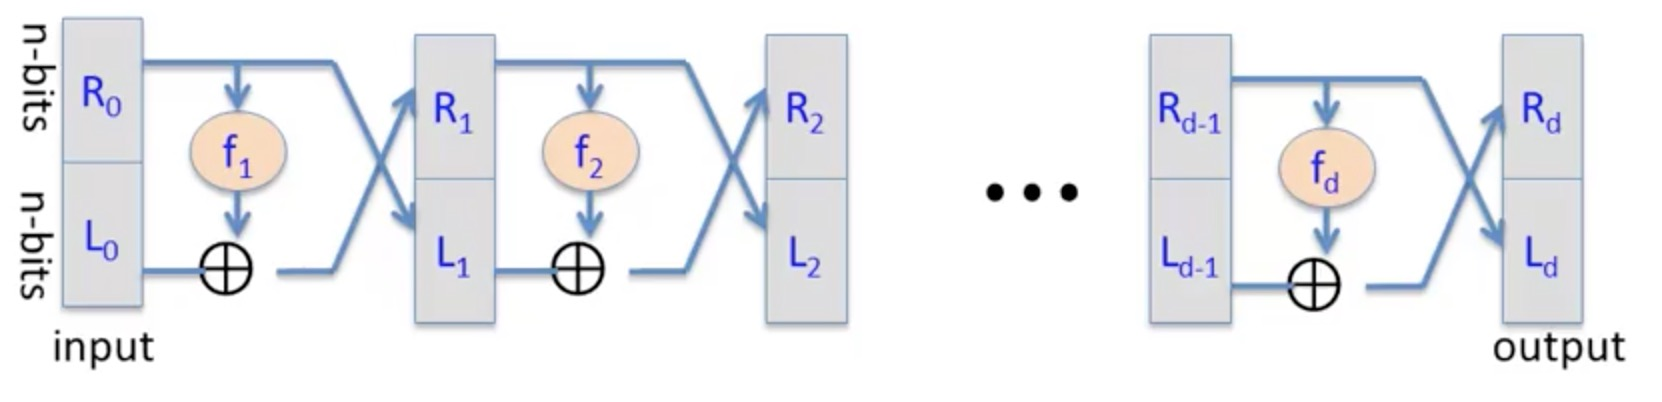
\includegraphics[width=\textwidth]{feistel.jpg}
\caption{Feistel Network}\label{feistel}
\end{figure}

It is easy to construct its inverse:
\begin{equation*}\begin{cases}
R_{i-1}&=L_i\\
L_{i-1}&=f_i(L_i)\oplus R_i
\end{cases}\end{equation*}
for $i=d,\dots,1$. Feistel network is used in many block ciphers, but not in AES.

The following theorem is important in the theory of DES. 
\begin{theorem}(Luby-Rackoff)\label{lubyrackoff}
If $f:K\times\{0,1\}^n\rightarrow\{0,1\}^n$ is a secure PRF, then a 3-round Feistel Network (Figure \ref{3rfeistel}) $F:K^3\times\{0,1\}^{2n}\rightarrow\{0,1\}^{2n}$ is a secure PRP.
\end{theorem}
\begin{figure}[ht]
\centering
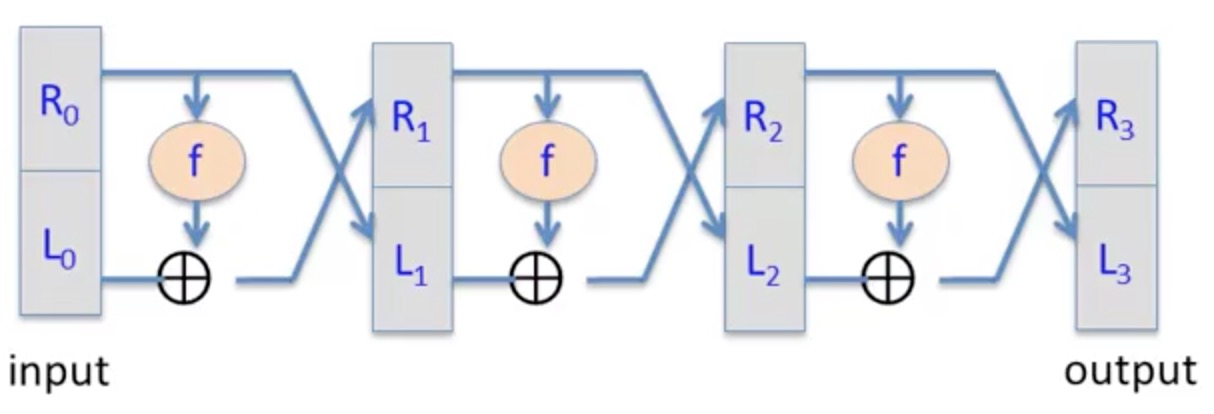
\includegraphics[width=\textwidth]{3rfeistel.jpg}
\caption{3-Round Feistel Network}\label{3rfeistel}
\end{figure}
The theorem means that if we have a secure PRF at hand, we can construct a secure block cipher.

DES is essentially a 16-round Feistel network. It uses 16 functions $F(k_i,x)=f_i(x):\{0,1\}^{32}\rightarrow\{0,1\}^{32},i=1,\dots,16$, as shown in Figure \ref{des}. IP is an initial permutator not for security reason, but required by the standard, and IP$^{-1}$ is its inverse. The Feistel network uses 16 48-bit keys expanded from a 56-bit initial key\footnote{We won't discuss the key expansion.}.
\begin{figure}[ht]
\centering
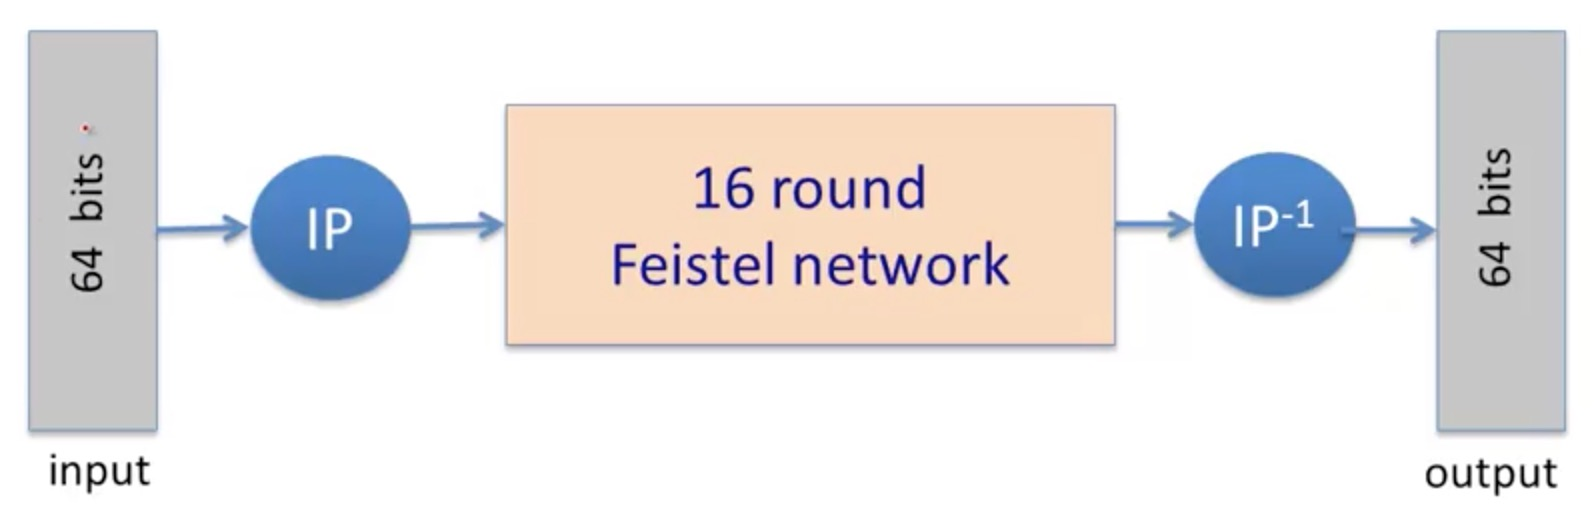
\includegraphics[width=\textwidth]{DES.jpg}
\caption{DES}\label{des}
\end{figure}
\subsection{DES Round Function}
Let's now discuss the round function $F(k_i,x)$. It carries out the following steps.
\begin{enumerate}
\item Pass the 32-bit input $x$ to an expansion box $E$, which expands it to 48 bits $x'$ by simply replicating and moving bits (i.e. linear operation that can be represented by a matrix)
\item Compute $x'\oplus k_i$ ($k_i$ is also 48 bits).
\item Break $x'\oplus k_i$ into 8 6-bit groups.
\item Each 6-bit group goes through an $S$ box and gets mapped to 4 bits.
\item Gather the 8 4-bit results and use a $P$ box to permute them into a 32-bit output.  
\end{enumerate}

The $S$ boxes are $\{0,1\}^6\rightarrow\{0,1\}^4$ functions implemented as lookup tables. Figure \ref{sboxeg} is an example.
\begin{figure}[ht]
\centering
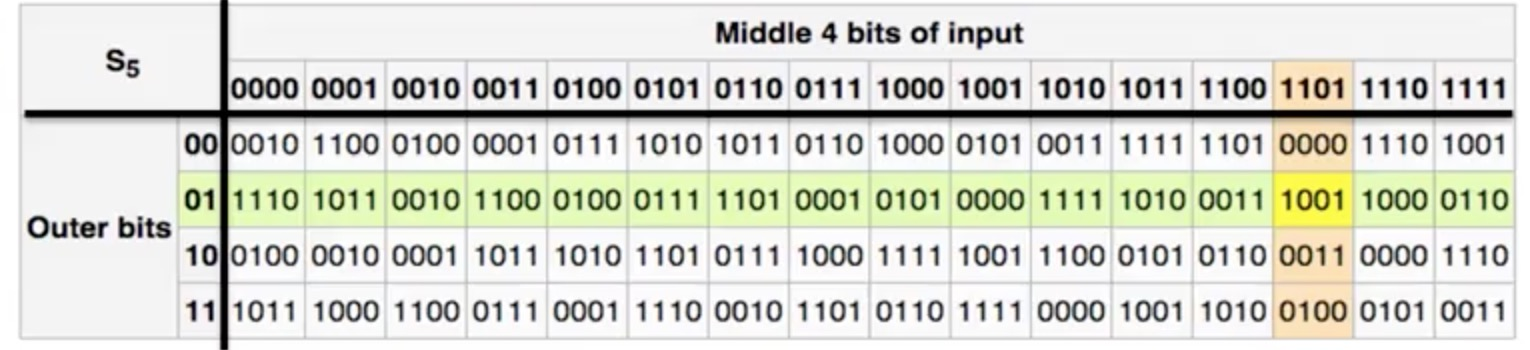
\includegraphics[width=\textwidth]{sboxeg.jpg}
\caption{An Example of $S$ Box}\label{sboxeg}
\end{figure}

The choice of these functions is subtle. For example, linear functions 
\[S_i(\vec{x})=A_i\cdot\vec{x}\pmod 2\]
with $A_i$ being a $4\times 6$ matrix are bad choices. One example could be 
\[\begin{pmatrix}
0 & 1 & 1 & 0 & 0 & 0 \\
1 & 0 & 0 & 1 & 1 & 0 \\
1 & 0 & 0 & 0 & 0 & 1 \\
0 & 1 & 1 & 0 & 0 & 1
\end{pmatrix}\cdot\begin{pmatrix}
x_1\\
x_2\\
x_3\\
x_4\\
x_5\\
x_6
\end{pmatrix} \pmod 2=\begin{pmatrix}
x_2\oplus x_3\\
x_1\oplus x_4 \oplus x_5\\
x_1\oplus x_6\\
x_2\oplus x_3\oplus x_6
\end{pmatrix}\]
The reason is that we can then find a $64\times 832$\footnote{832 = 64 + 48 * 16} matrix $B$ such that 
\begin{align*}
DES(k,m)&=B\cdot\begin{pmatrix}m&k_1&\cdots&k_{16}\end{pmatrix}^{\mathsf{T}}\coloneqq B\cdot\begin{pmatrix}m\\\mathcal{K}\end{pmatrix}\\
&=m_{i_1}\oplus\cdots\oplus m_{i_n}\oplus \mathcal{K}_{j_1}\oplus\cdots\oplus \mathcal{K}_{j_k},
\end{align*}
i.e DES as a whole becomes linear. Then we have 
\begin{align*}
 &DES(k,m_1)\oplus DES(k,m_2)\oplus DES(k,m_3)\\
=&B\cdot\begin{pmatrix}m_1\\\mathcal{K}\end{pmatrix}\oplus B\cdot\begin{pmatrix}m_2\\\mathcal{K}\end{pmatrix}\oplus  B\cdot\begin{pmatrix}m_3\\\mathcal{K}\end{pmatrix}\\
=&B\cdot\begin{pmatrix}m_1\oplus m_2\oplus m_3\\\mathcal{K}\end{pmatrix}\\
=&DES(k,m_1\oplus m_2\oplus m_3),
\end{align*}
which is not a property that holds for a random function, and thus makes DES insecure. What's worse, all round keys can be extracted given 832 $m-c$ pairs.

It has been proven that even choosing the $S$ boxes and $P$ box at random will result in an insecure block cipher. There are a lot of rules limiting the choices in order to guarantee the security of DES.
\section{Attacks on DES}
\subsection{Exhaustive Search Attack}
The goal of an \textbf{exhaustive search attack} is to recover the key $k$ given 3 input-output pairs $m_i,c_i=E(k,m_i),i=1,2,3.$ We use ``the'' key because the following lemma convinces us of its uniqueness.
\begin{lemma}
Suppose DES is an \textbf{ideal cipher}\footnote{This is idealized, not the actual situation}, i.e. DES is a collection of $2^{56}$ random invertible functions 
\[\pi_i:\{0,1\}^{64}\rightarrow\{0,1\}^{64},i=1,\dots,2^{56}.\]
Then $\forall m,c$, 
\[Pr(\text{at most one key s.t. $c=DES(k,m)$})\geq 1-\frac{1}{256}\approx 99.5\%.\]
\end{lemma}
\begin{proof}
\begin{align*}
&Pr(\exists k'\neq k\:s.t.\:c=DES(k,m)=DES(k',m))\\
\leq&\sum\limits_{k'\in\{0,1\}^{56}}Pr(DES(k',m)=c)\\
=&2^{56}\cdot\frac{1}{2^{64}}=\frac{1}{256}
\end{align*}
\end{proof}
This fact makes it possible to find the $k$ with brute force search with only one $m-c$ pair. It is not that difficult to use modern computers to do this with a 56-bit cipher, so 56-bit DES ciphers should no longer be used. 

There are ways to enhance the security of DES. 
\subsubsection{3DES}
Let $E:K\times M\rightarrow M$ be a 56-bit DES cipher. The define a 3DES cipher $3E:K^{3}\times M\rightarrow M$ as 
\[3E((k_1,k_2,k_3),m)=E(k_1,D(k_2,E(k_3,m))).\]
3DES has the key size of $56\times 3=168$. It is safer than DES, but it is also 3 times slower. We use E-D-E instead of E-E-E in order to be able to produce DES result with $k_1=k_2=k_3$.

The reason to use 3DES instead of 2DES is that 2DES is breakable with less time than it appears to need, making it insecure. Define 
\[2E((k_1,k_2,k_3),m)=E(k_1,E(k_2,m)).\]
Given a $m-c$ pair, we have 
$E(k_1,E(k_2,m))=c$, therefore $D(k_1,c)=E(k_2,m)$, which inspires us of a new way to break the cipher, namely the meet-in-the-middle attack. 

First we calculate $E(k_i,m)$ for all $2^{56}$ possible keys and save them in a table. Then we sort the table according to the value of $E(k_i,m)$. Finally for each possible $k_i$, we calculate $D(k_i,c)$ and search for it in the table. Building and sorting the table takes $2^{56}\log(2^{56})$ time. Searching for all the decryptions takes another $2^{56}\log(2^{56})$ time. In total the time consumption is smaller than $2^{63}\ll 2^{112}$, making 2DES insecure.

The same strategy can be used to break 3DES in $2^{118}$ time:
\[2^{56}\log(2^{56})+2^{56\times 2}\log(2^{56})=2^{118}.\]
\subsubsection{DESX}
Define DESX cipher $EX:K^{3}\times M\rightarrow M$ as 
\[EX((k_1,k_2,k_3),m)=k_1\oplus E(k_2,k_3\oplus m).\]
It has a key length of 64+56+64=184. A meet-in-the-middle attack takes $2^{120}$ time: using $k_1\oplus c=E(k_2,k_3\oplus m)$, the time consumption is 
\[2^{56+64}\log(2^{56+64})+2^{64}\log(2^{56+64})=2^{120}.\]

Nonetheless, if only one XOR is used, i.e. $k_1$ or $k_3$ is not used, the cipher will be no securer than DES.
\subsection{Side Channel Attacks}
An attacker can obtain the key by precisely measuring the time or power consumption of encryption/decryption. If the cipher is run in one of the cores of a multi-core processor, an attacker can obtain the key by counting the number of cache misses in the shared cache. 
\subsection{Fault Attack}
An error in the last round can expose the secret key. Thus the correctness of the algorithm needs to be guaranteed, which serves as a strong reason for us not to attempt to implement cryptography primitives.
\subsection{Linear/Differential Attacks}
The goal is to recover the key in less than $2^{56}$ time when given many $m-c$ pairs. Suppose for random $k,m$, 
\[Pr((m[i_1]\oplus\cdots\oplus m[i_r])\oplus(c[j_1]\oplus\cdots\oplus c[j_r]) = k[l_1]\oplus\cdots\oplus k[l_r])=\frac{1}{2}+\epsilon\]
holds for some non-zero $\epsilon$, in which $m[i_1]\dots m[i_r]$ is a subset of the message bits, $c[j_1]\dots c[j_r]$ is a subset of the cipher text bits, and $k[l_1]\dots k[l_r]$ is a subset of the key bits, then we have the following theorem.
\begin{theorem}
Given $\frac{1}{\epsilon^2}$ random $m-c$ pairs, then we have
\[k[l_1]\oplus\cdots\oplus k[l_r]=mode((m[i_1]\oplus\cdots\oplus m[i_r])\oplus(c[j_1]\oplus\cdots\oplus c[j_r]))\]
with a probability $\geq 97.7\%$.
\end{theorem}
Mode is the statistical mode: element with maximum frequency. 

For DES, we have $\epsilon=\frac{1}{2^{21}}$. With $2^{42}$ $m-c$ pairs we can find 14 key bits in time $2^{42}$. Then we can do a brute force search for the remaining bits in $2^{42}$ time, thus the overall attack time is $2^{43}\ll 2^{56}$. 

This is another reason against implementing our own ciphers: a little bias of the cipher leads to an easy attack.
\subsection{Quantum Attacks}
Consider a generic problem: given $f:X\rightarrow\{0,1\}$ that is a function evaluating to 0 most of the time, try to find $x\in X$ s.t. $f(x)=1$. On a classical computer, the best generic algorithm takes $O(\lvert X\rvert)$ time. A quantum on the contrary can solve the problem in $O(\sqrt{\lvert X\rvert})$ time.

To attack a block cipher, we can use the function
\begin{equation*}
f(k)=\begin{cases}
1&if\:E(k,m)=c\\
0&otherwise
\end{cases}\end{equation*}
This means that a quantum search algorithm can find the key in $O(\sqrt{\lvert K\rvert})$ time. For DES this means $2^{28}$ time. 

\section{Advanced Encryption Standard(AES)}
AES is built as a substitution-permutation network (Figure \ref{aes_network}). In each round, the input is first XOR'ed with a round key, then goes through a substitution layer in which blocks of the state are substituted according to the substitution table, and finally goes through a permutation in which bits are permuted and shuffled around. Every step must be reversible so that the whole algorithm is reversible. The decryption process is simply all the steps taken in reverse order. Specifically, Figure \ref{aes128} shows the process of AES 128 encryption.

\begin{figure}[ht]
\centering
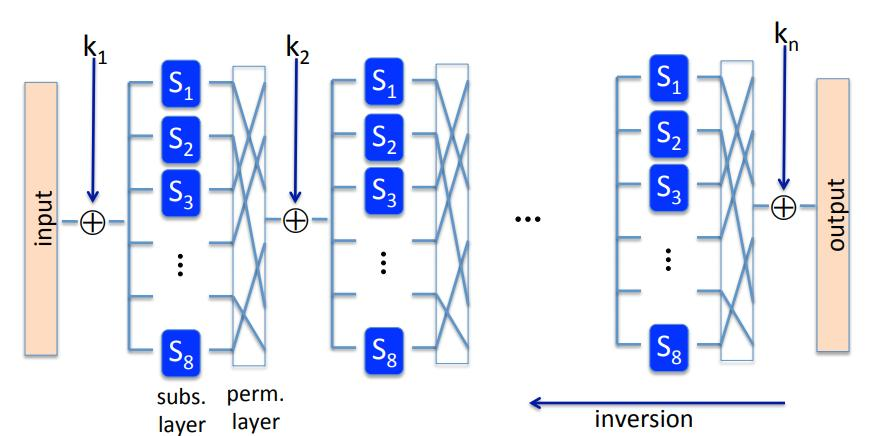
\includegraphics[width=\textwidth]{AES_network.jpg}
\caption{AES Subs-Perm Network}\label{aes_network}
\end{figure}
\begin{figure}[ht]
\centering
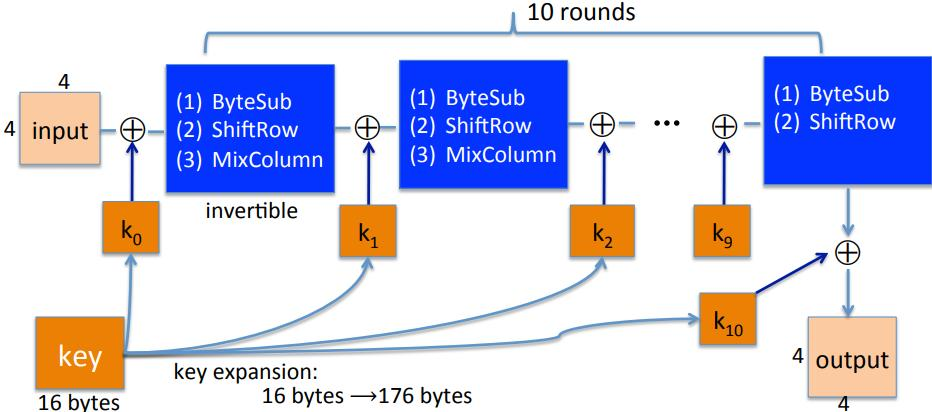
\includegraphics[width=\textwidth]{aes128.jpg}
\caption{AES 128 Schematic}\label{aes128}
\end{figure}

The 16-byte input is written as a 4$\times$4 matrix $A$. The first function $ByteSub$ is just a 1-byte S-box that maps a byte to another:
\[A[i,j]\rightarrow S[A[i,j]],\forall i,j.\]
The second function $Shiftrow$ does a cyclic shift on each row:
\begin{equation*}
\begin{bmatrix}
  S_{00} & S_{01} & S_{02} & S_{03} \\ 
  S_{10} & S_{11} & S_{12} & S_{13} \\ 
  S_{20} & S_{21} & S_{22} & S_{23} \\ 
  S_{30} & S_{31} & S_{32} & S_{33} \\ 
\end{bmatrix}\Rightarrow
\begin{bmatrix}
  S_{00} & S_{01} & S_{02} & S_{03} \\ 
  S_{11} & S_{12} & S_{13} & S_{10} \\ 
  S_{22} & S_{23} & S_{20} & S_{21} \\ 
  S_{33} & S_{30} & S_{31} & S_{32} \\ 
\end{bmatrix}.
\end{equation*}
The third function $MixColumn$ applies a linear function on each column. All 3 steps are easily computable, allowing AES to be implemented with no pre-computation (thus small code size). There is a tradeoff between code size and performance: the smaller the code size, the slower the implementation is. The javascript AES lib makes use of this fact to accelerate both code transmission through web and local computation in the browser: code with no pre-computation is transmitted from server to the browser, and pre-compute tables are computed prior to encryption.

Two types of attacks are known to exist for AES: the best key recovery attack on AES-128 (4 times faster than brute-force search, $2^{126}$) and the related key attack on AES-256 (much faster than brute-force search, $2^{99}$). 
\section{Block Ciphers from PRGs}
Let $G:K\rightarrow K^2(G(k)=G(k)[0]\parallel G(k)[1]$) be a PRG, and define a 1-bit PRF $F:K\times\{0,1\}\rightarrow K$ as 
\[F(k,x)=G(k)[x], x\in\{0,1\}.\]
Then obviously we have
\begin{theorem}
If $G$ is a secure PRG, then $F$ is a secure PRF.
\end{theorem}
\begin{figure}[ht]
\centering
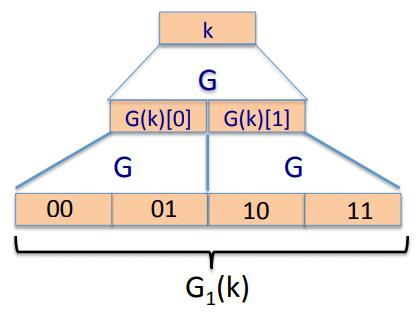
\includegraphics[width=0.5\textwidth]{prg2prf_g1.jpg}
\caption{PRG to PRF on $\{0,1\}^2$}\label{prg2prf_g1}
\end{figure}
$G,F$ can be extended to get $G_1:K\rightarrow K^4, F_1:K\times\{0,1\}^2\rightarrow K$, as shown in Figure \ref{prg2prf_g1}. The security of $G_1$ can be proved according to the security of $G$.
\begin{align*}
G_1(k)&=G(G(k)[0])\parallel G(G(k)[1])\\
F_1(k, x)&=G_1(k)[x]
\end{align*}

We can extend more and more to obtain a secure PRF(the GGM PRF) on $K\times\{0,1\}^n$.
\begin{align*}
\begin{cases}
  k_1&=G(k)[x_0]\\
k_2&=G(k1)[x_1]\\
&\cdots\\
k_n&=G(k_{n-1})[x_{n-1}]\\
\end{cases}\\
F(k,x_0x_1\cdots x_{n-1})=k_n\\
\end{align*}
According to Theorem \ref{lubyrackoff}, a $2n$ bit PRP can be obtained from the PRF, thus a block cipher can be defined. This secure PRF and the block cipher it defines is not used in practice because it is too slow ($n$ times slower than the original PRG).
\ifx\PREAMBLE\undefined
\end{document}
\fi
% \clearpage%somehow needed so that list of algorithms in toc jumps to the correct page.
% \phantomsection
% \addcontentsline{toc}{chapter}{\listtheoremname}
% \listoftheorems[ignoreall, show={definition}]
\end{document}